\documentclass{standalone}
%% Show/hide steps for standalone work — edit this line:
\makeatletter\AtBeginDocument{\@buildstepset{1,2,3,4,5,6,7,8,9,10}}\makeatother
\usepackage{graphicx}
\usepackage{tikz}
\usepackage{hsbcommon}
\begin{document}
    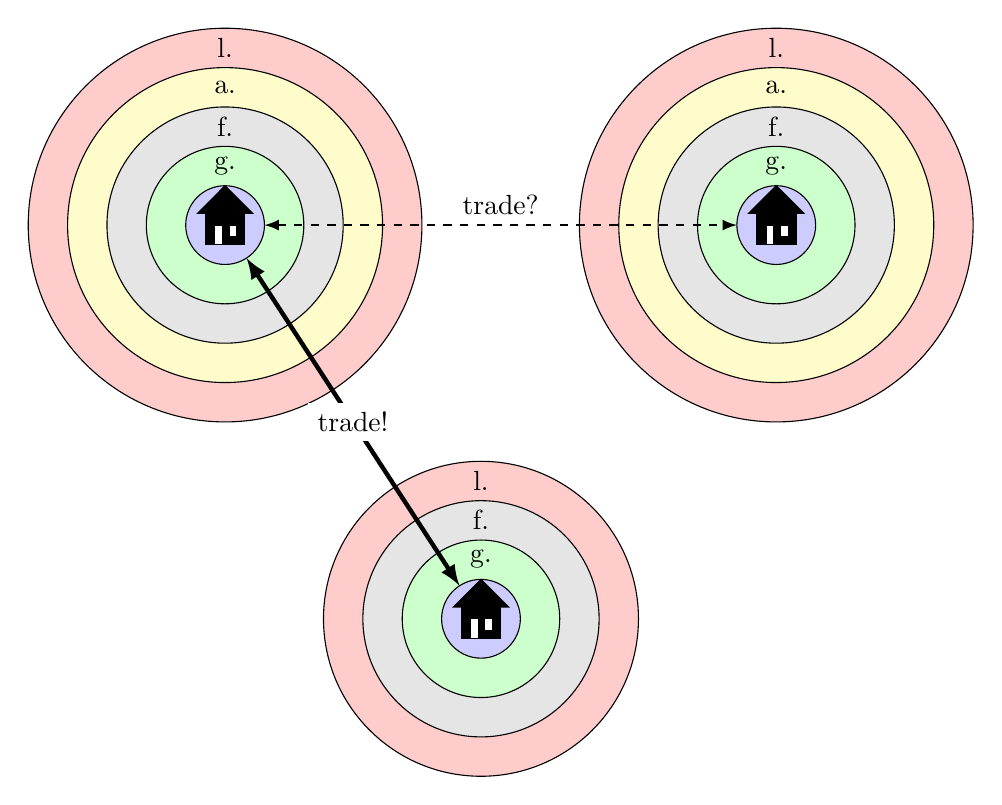
\begin{tikzpicture}
    \tikzset{
        myhome/.pic={
        \begin{scope}[xshift=-0.25cm,yshift=-0.25cm]         
            \filldraw (0,0) rectangle (0.5,0.4);
            \filldraw (-0.1,0.4) -- (0.25,0.75) -- (0.6,0.4) -- cycle;
            \filldraw[white,draw=black] (0.12,0) rectangle (0.22,0.25);
            \filldraw[white,draw=black] (0.3,0.1) rectangle (0.4,0.25);
        \end{scope}
        }
    }
    \tikzset{
        myrings/.pic={
        \foreach [count=\i] \ii/\mycol in 
        {
            l/red,
            a/yellow,
            f/gray,
            g/green,
            /blue%
        }
        {
            \draw[fill=\mycol!20] (0:0) circle (6-\i);
            \node at (90:6-\i-0.5) {\ii.};
        }
        \draw (0,0) pic {myhome};
        }
    }
    \tikzset{
        myringsdiff/.pic={
        \foreach [count=\i] \ii/\mycol in 
        {
            l/red,
            f/gray,
            g/green,
            /blue%
        }
        {
            \draw[fill=\mycol!20] (0:0) circle (5-\i);
            \node at (90:5-\i-0.5) {\ii.};
        }
        \draw (0,0) pic {myhome};
        }
    }
    \coordinate (1st) at (-3.5,0);
    \coordinate (2nd) at ( 3.5,0);
    \draw (1st) pic[scale=0.5] {myrings};
    \draw (2nd) pic[scale=0.5] {myrings};
    \draw[<->,dashed,thick,>=latex,shorten >=.5cm, shorten <=.5cm] (1st) -- node[above] {trade?} (2nd);

    \ifstep{2}{
\begin{scope}[yshift=-5cm,xshift=3.25cm]

        \coordinate (3rd) at (-3.5,0) ;
        \draw (3rd) pic[scale=0.5] {myringsdiff};
        \ifstep{3}{\draw[<->,ultra thick,>=latex,shorten >=.5cm, shorten <=.5cm] (3rd) -- node[fill=white] {trade!} (1st);}
    \end{scope}
}



    \end{tikzpicture}
\end{document}